\mychapter{Funcions elementals}{Funcions elementals}{
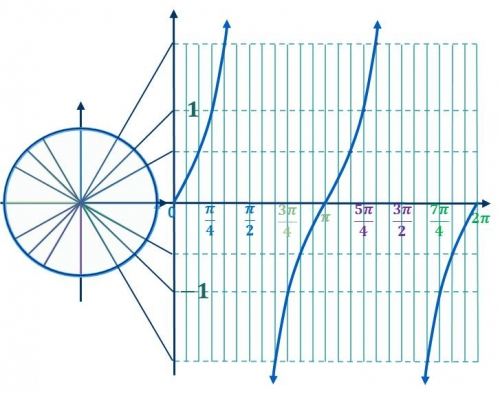
\includegraphics[width=4.5cm]{img-05/chap6.jpg}
}{chap:elemental}

 \vspace*{\fill}
 
\begin{blueshaded}
	
	{\Large \textbf{Una breu història}}
	
	
	\begin{wrapfigure}{R}{4cm}
		\begin{center}
		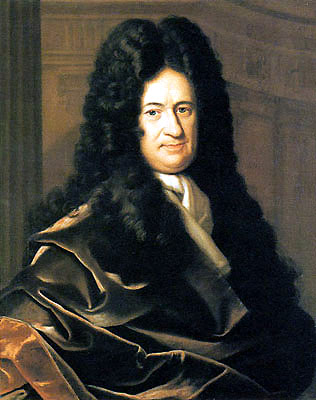
\includegraphics[width=3cm]{img-05/leibniz.jpg}	
		{\footnotesize
		Gottfried Leibniz va introduir el terme «funció» en el segle XVII.}
		\end{center}
	\end{wrapfigure}
	El concepte de funció com el coneixem avui en dia, va aparèixer amb als inicis del càlcul en el segle XVII. René Descartes, Isaac Newton i Gottfried Leibniz van establir la idea de funció com la dependència entre dues quantitats. Leibniz, en particular, va introduir els termes «Funció», «variables», «constant» i «paràmetre». La notació $f(x)$ va ser utilitzada per primera vegada per A.C. Clairaut i per Leonhard Euler en la seva obra {\normalfont \textit{Commentarii de Sant Petersburg}} en 1736.
	
	Inicialment, una funció $f$ s'identificava a efectes pràctics amb una expressió analítica que permetia calcular els seus valors. No obstant això, aquesta definició tenia algunes limitacions: Expressions analítiques diferents podien donar lloc a valors numèrics iguals. En 1837, Dirichlet va proposar la definició moderna de funció com una correspondència entre dos conjunts de nombres, que associa a cada nombre del conjunt de sortida un únic nombre del conjunt d'arribada.
	 
\end{blueshaded}


 \vspace*{\fill}
 
\newpage
\heading{Prova inicial}

Associa a cada gràfica una equació de les que es presenten a continuació.

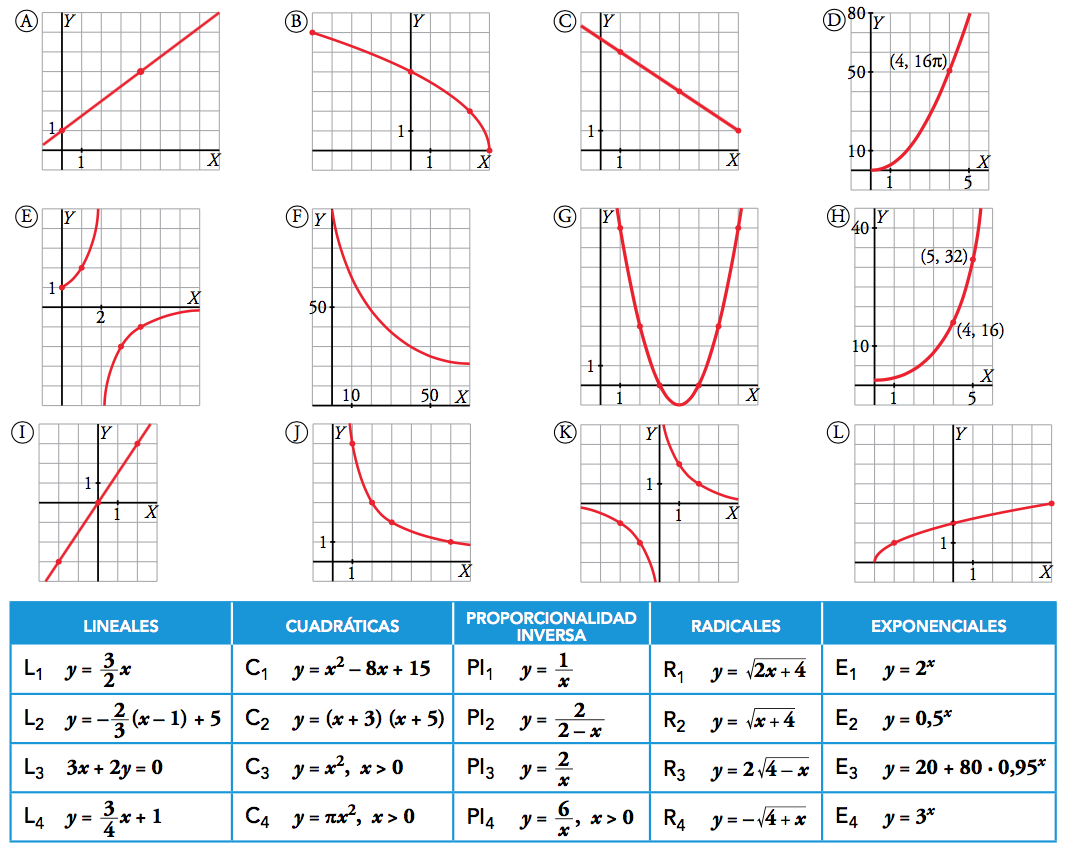
\includegraphics[width=\textwidth]{img-05/chap6-inicial.png}

\addanswersline[cols=1]{Avaluació inicial}{0}{
\begin{tasks}(4)
	\task L$_{4}$	\task R$_3$		\task L$_2$		\task C$_4$
	\task PI$_{2}$	\task E$_3$		\task C$_1$		\task E$_1$
	\task L$_{1}$	\task PI$_4$		\task PI$_3$		\task R$_2$
\end{tasks}
\par
No tenen gràfica associada L$_3$, C$_2$, C$_3$, PI$_1$, R$_1$, R$_4$, E$_2$ i E$_4$. 
}

\section{Concepte de funció}

\begin{theorybox}
	$f: Dom \rightarrow Rec$ és una funció si per a cada $x$ del domini $Dom$ associa \textbf{un únic} valor $y$ del recorregut $Rec$. S'anomena $y=f(x)$, la imatge de $x$ per la funció $f$.
	
	Si $Dom\, f$ són els nombres naturals, parlam de \textbf{successions}.
	
	Si $Dom\, f$ és el conjunt dels nombres reals, parlam de \textbf{funcions de variable real}.
	
	
	Per representar funcions utilitzam uns eixos cartesians on col·locam $x$ sobre l'eix horitzontal (\textbf{abscisses}) i $y$ sobre l'eix vertical (\textbf{ordenades}).
\end{theorybox}

\subsection{Successions}
\begin{theorybox}
	Una successió és una llista ordenada de nombres reals que anomenam termes:
	\[ a_n : a_1, a_2, a_3, \cdots \]
	
	Una successió es pot expressar:
	\begin{itemize}
		\item Donant els primers termes: $1, 3, 5, 7, \cdots$
		\item Donant el terme general: $a_n = 2n-1$
		\item Donant una relació de recurrència: $a_1 = 1$ i $a_{n+1}=a_n+2$
	\end{itemize}
\end{theorybox}

\begin{mylist}
\exer[1]	Troba els 7 primers termes de la successió $a_1=2$, $a_2=3$, $a_n=a_{n-1
	}+a_{n-2}$.	
\answers{2, 3, 5, 8, 13, 21, 34, ...}

\exer[1] Dóna el terme general o la relació de recurrència de les successions:
\begin{tasks}
	\task $3, 8, 13, 18, 23, \cdots$
	\task $1, 8, 27, 64, 125, \cdots$
	\task $8, 4, 2, 1, \cdots$
\end{tasks}

\answers{a) $a_n=3+5(n-1)$ o $a_1=3$ $a_n=a_{n-1}+3$ \par b) $a_n=n^3$ \par c) $a_n=8\cdot (1/2)^{n-1}$ o $a_1=8$ $a_n=a_{n-1}/2$]}
\end{mylist}

\begin{theorybox}[Progressions aritmètiques]
	Una progressió aritmètica és una successió en la qual la diferència $d$ entre dos termes consecutius es manté constant.
	
	El terme general és: $a_n = a_1 + d \cdot (n-1)$.
	
	La suma dels $N$ primers termes és: $S_N = \dfrac{a_1+a_N}{2} \cdot N$
\end{theorybox}
 

\begin{theorybox}[Progressions geomètriques]
		Una progressió geomètrica és una successió en la qual el quocient (anomenat raó $r$)  entre dos termes consecutius es manté constant.
	
	El terme general és: $a_n = a_1 \cdot r^{n-1}$.
	
	La suma dels $N$ primers termes és: $S_N = a_1 \dfrac{r^N-1}{r-1}$
	
	Si $|r|<1$, la progressió és decreixent i la suma dels infinits termes és: $S_\infty = \dfrac{a_1}{1-r}$
\end{theorybox}

\begin{mylist}
	\exer[1] Troba el terme 100 de la progressió $10, 7, 4, 1, -2, \cdots$.
	\answers{$a_n=10-3(n-1)$ i $a_{100}=-197$}
	
	\exer[1] D'una progressió aritmètica coneixem $a_3=11$ i $a_5=19$. Calcula el terme general i la suma dels 100 primers termes.
	\answers{$d=(19-11)/2=4$ i $a_1=3$, \linebreak $a_n=3+4(n-1)$, $S_{100}=20100$}
	
	\exer[1] Troba el terme 50 de la progressió $100, 50, 25, 12.5, \cdots$. Troba la suma dels infinits termes.
	\answers{$a_n=100\cdot(0.5)^{n-1}$, $a_{50}=1.776\cdot 10^{-13}$, $S_\infty=200$}
	
	\exer[1] Calcula la suma dels 30 primers termes d'una progressió geomètrica amb termes \linebreak $a_2=3$ i $a_5=81$.
	\answers{$r=3$ i $a_1=1$, $a_n=3^{n-1}$, $S_{30}=1.029\cdot 10^{14}$}
	
\end{mylist}

\subsection{Funcions de variable real}

\begin{mylist}

\begin{minipage}[T]{0.58\textwidth}
	\exer Quines d'aquestes gràfiques representen funció i quines no? Explica per què?	
\end{minipage}
\begin{minipage}{0.38\textwidth}
	\noindent 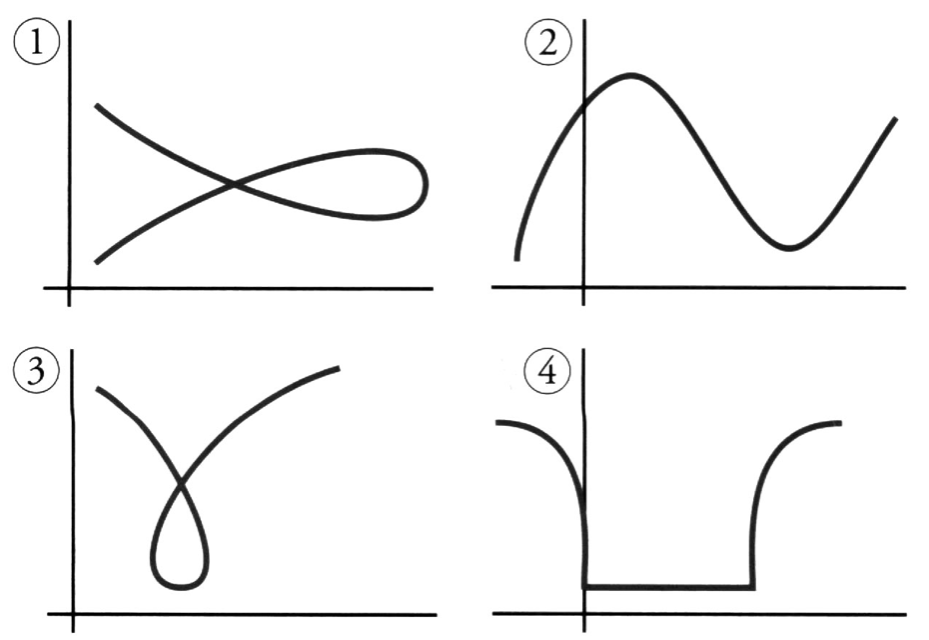
\includegraphics[width=0.85\textwidth]{img-05/fe-is-func}	
\end{minipage}
 \answers{Són funcions 2 i 4. No són funcions 1 i 3, perquè per un mateix valor de $x$ trobam més d'un valor de $y$ ``La gràfica té plegaments''.}	

\exer \mental Observa les gràfiques d'aquestes funcions i indica quin és el seu domini de definició i el seu recorregut:	

\noindent 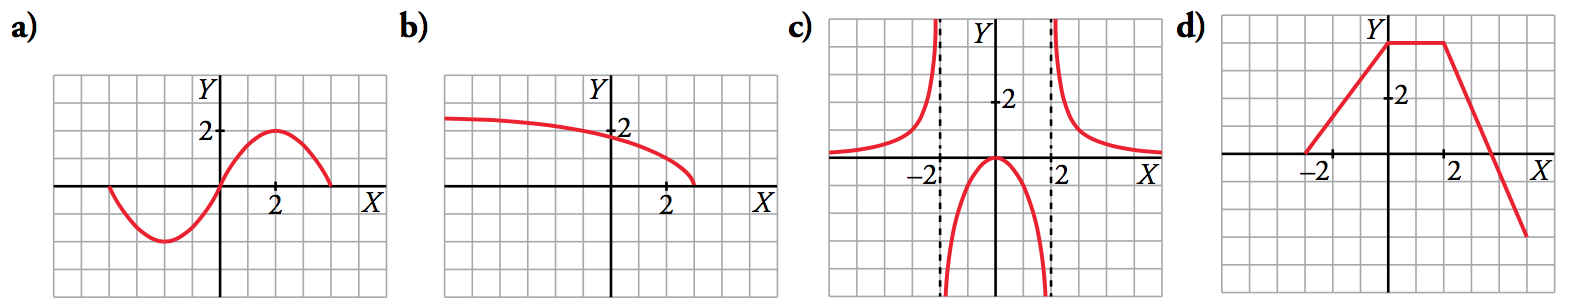
\includegraphics[width=0.93\textwidth]{img-05/fe-dom-rec}	
\answers{[Dom $f=[-4,4]$, Dom $f=(-\infty,3)]$, Dom $f=(-\infty,-2)\cup(-2,2)\cup (2,+\infty)$ o també  Dom $f=\Re-\{-2,2\}$, Dom $f=[-2,5]$]}
\end{mylist}

\begin{theorybox}
	Totes les funcions polinòmiques tenen com $Dom f=\mathbb{R}$. Però, hi ha situacions en què el domini es troba limitat perquè és impossible calcular la funció.
	\begin{itemize}
		\item No és possible dividir entre zero.
		\item No es pot calcular l'arrel quadrada d'un nombre negatiu.
		\item No existeix el logaritme de zero ni d'un nombre negatiu.
		\item No té sentit físic; per exemple no existeixen àrees negatives.
	\end{itemize}
\end{theorybox}

\begin{resolt}[E]{Calcula el domini de \par
		  $y=\dfrac{x}{x^2-4}$
	}
  El denominador és igual a zero quan $x=\pm 2$, el domini són tots els nombres reals excepte aquests dos: $Dom\, f=\mathbb{R}-\{-2,2\}$
\end{resolt}  
\vspace{-0.75cm}
\begin{resolt}{Calcula el domini de 	\begin{equation*}
	y=\sqrt{3-x}
		\end{equation*}  }
 El radicand ha d'esser major o igual a zero $3-x \geq 0$. La solució d'aquesta inequació és $x\leq 3$ o en forma d'interval $Dom\, f=(-\infty, 3]$
\end{resolt}  
\vspace{-0.75cm}
\begin{resolt}{Calcula el domini de 	\begin{equation*}
	y=\sqrt{\dfrac{x+2}{x-1}}
		\end{equation*}}
	  En primer lloc el denominador no pot ésser zero; llavors $x=1$ queda descartat. En segon lloc, el radicand ha d'esser major o igual a zero. Per això analitzam els signes del numerador i denominador:
	\begin{center}
		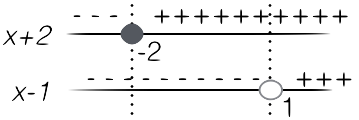
\includegraphics[width=0.32\textwidth]{img-05/chap-fe-domsignes.png}
	\end{center}
	
	El signe de la divisió ha de donar positiu o zero, aleshores $Dom f=(-\infty, -2] \cup (1, +\infty)$.
\end{resolt}

\begin{mylist} 
	
	
	\exer[1]  Calcula en el teu quadern el domini de les següents funcions:
	
	
	\begin{tabular}{|p{0.2in}|p{0.9in}|p{1.3in}|p{0.2in}|p{0.8in}|p{1.4in}|} \hline 
		\multicolumn{2}{|p{1in}|}{\textbf{Funció}} & \textbf{Domini} & \multicolumn{2}{|p{1.0in}|}{\textbf{Funció}} & \textbf{Domini} \\ \hline 
		\textit{f} & $\dfrac{5x^{2} +1}{x^{2} -4} $ &  &  \textit{j} & $\sqrt{\frac{x+3}{x-3} } $ &  \\ \hline 
		\textit{g} & $\sqrt{\frac{3x+2}{x-3} } $ &  &  \textit{k} & $\dfrac{2x^{2} -1}{x^{2} -3} $ &  \\ \hline 
		\textit{h} & $\dfrac{x+1}{x-1} $ &  &  \textit{l} & $\sqrt{\frac{x+2}{3-x} } $ &  \\ \hline 
		\textit{i} & $\dfrac{x^{2} +1}{x^{2} -1} $ &  &  \textit{m} & $\dfrac{x+1}{x-1} $ &  \\ \hline 
	\end{tabular}
\answers{$\text{Dom }f=\Re-\{\pm 2\}$,\par $\text{Dom } g=(-\infty,-2/3]\cup (3,+\infty)$,\par $\text{Dom } h=\Re-\{1\}$,\par $\text{Dom } i=\Re-\{\pm 1\}$,\par $\text{Dom } j=(-\infty,-3]\cup(3,+\infty)$,\par $\text{Dom } k=\Re-\{\pm \sqrt{3}\}$,\par $\text{Dom } l=[-2,3)$, $\text{Dom } m=\Re - \{1\}$}
	
\exer Calcula en el teu quadern el domini de cadascuna de les següents funcions:
\[\begin{array}{lll} 
p(x)=-5x+3;&q(x)=\sqrt{2x^{2} -x+7}&;r(x)=\sqrt[{4}]{-x^{3} -1} \\ s(x)=\sqrt[{3}]{3x^{2} -x};&f(x)=\dfrac{2x-4}{x+3};&\quad g(x)=\dfrac{-3}{x} \\ 
h(x)=\dfrac{x+1}{x^{2} +1};& j(x)=\dfrac{-x^{2} +2x}{x^{2} -4}& \end{array}\] 
 
\begin{tabular}{|p{0.2in} p{0.6in}|p{1.5in}|p{0.3in} p{0.6in} | p{1.6in}|} \hline 
\multicolumn{2}{|p{1in}|}{Funció} & Domini & \multicolumn{2}{|p{0.9in}|}{Funció} & Domini \\ \hline 
\textit{} & $p(x)$ &  &  \textit{} & $q(x)$ &  \\ \hline 
\textit{} & $r(x)$ &  &  \textit{} & $s(x)$ &  \\ \hline 
\textit{} & $f(x)$ &  &  \textit{} & $g(x)$ &  \\ \hline 
\textit{} & $h(x)$ &  &  \textit{} & $j(x)$ &  \\ \hline 
\end{tabular}

\answers{Dom $p=\Re$;\par Dom $q=\Re$;\par Dom $r=(-\infty,-1]$;\par Dom $s=\Re$;\par Dom $f=\Re-\{-3\}$;\par Dom $g=\Re-\{0\}$;\par Dom $h=\Re$;\par Dom $j=\Re-\{-2,2\}$ }

\exer Sigui la funció donada per $f\left(x\right)=x^{3} +ax^{2} +bx+c$. Determina $a$, $b$ i $c$ sabent que la funció té simetria senar i que passa pel punt (1, $-2$).

\answers{Si és senar $a=0$ i $c=0$. Si passa per $(1,-2)$ implica que $b=-3$}

\exer  Les dades de la taula indiquen en la primera fila, els preus, en euros, per sac de taronges, en la segona fila, les quantitats demandades de taronges per setmanes, i en la tercera fila, les quantitats ofertes:

\begin{tabular}{|p{2.4in}|p{0.6in}|p{0.6in}|p{0.6in}|p{0.6in}|} \hline 
	Preu per sac (euros) & 8 & 6 & 4 & 2 \\ \hline 
	Quantitat demandada (milers de sacs per setmana) & 50 & 100 & 200 & 400 \\ \hline 
	Quantitat oferta (milers de sacs per setmana) & 300 & 250 & 200 & 100 \\ \hline 
\end{tabular}

Dibuixa una gràfica amb les dades d'aquesta taula, representant en l'eix vertical els preus, i en l'eix horitzontal les quantitats demandades i ofertes. Uneix amb un traç continu ambdues corbes.

\answers{Gràfica:\par 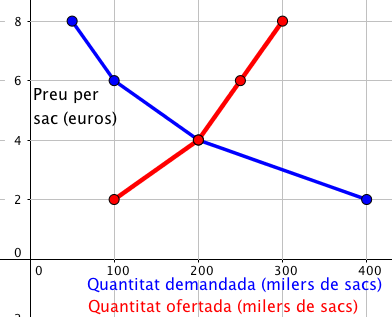
\includegraphics[width=0.4\textwidth]{img-sol/t5-12}}

\exer  Les dades de la taula indiquen en la primera fila, els preus, en euros, del lloguer d'un pis de 70 m${}^{2}$, en la segona fila, la quantitat de persones que desitgen llogar un pis, i en la tercera fila, els pisos buits en una determinada ciutat:


\begin{tabular}{|p{2.5in}|p{0.6in}|p{0.6in}|p{0.6in}|} \hline 
	Preu d'un pis (euros) & 1500 & 1000 & 500 \\ \hline 
	Quantitat demandada (persones que desitgen llogar) & 10 & 100 & 500 \\ \hline 
	Quantitat oferta (pisos lliures) & 600 & 200 & 50 \\ \hline 
\end{tabular}

\begin{tasks}
	\task  Dibuixa una gràfica de les corbes d'oferta i demanda.
	%%
	\task  Determina de forma aproximada el punt d'equilibri
\end{tasks}

\answers{a) Gràfica:\par 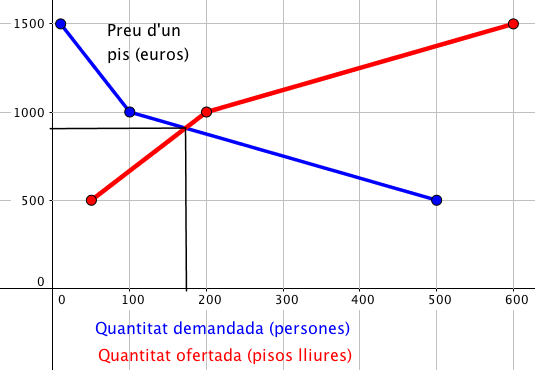
\includegraphics[width=0.4\textwidth]{img-sol/t5-13}\par b) El punt d'equilibri és quan l'oferta iguala la demanda. Això passarà per una oferta de 175 pisos  un preu per pis de 910 \euro{}.}



\end{mylist}

\section{Funcions elementals}
\vspace{-0.6cm} 
\subsection{Lineals i Quadràtiques}
\vspace{-0.4cm}
\begin{theorybox}[Funció lineal]
	L'expressió d'una funció lineal és $y=mx+n$, essent $m$ el pendent i $n$ l'ordenada a l'origen. Si $m=0$ es diu que la funció és constant i la gràfica és una recta horitzontal.
\end{theorybox}

\begin{theorybox}[Funció quadràtica o paràbola]
	L'expressió d'una funció quadràtica és $y=ax^2+bx+c$. Quan $a>0$ la funció és còncava $\cup$ i si $a<0$ és convexa $\cap$. El valor de $b$ controla la posició del vèrtex. L'abscissa del vèrtex s'obté de la fórmula $x_v=\dfrac{-b}{2a}$. L'ordenada del vèrtex es troba substituïnt $x_v$ dins la funció.
\end{theorybox}


\begin{mylist}
\exer Calcula el vèrtex i punts de talls amb els eixos de les següents paràboles. Representa-les gràficament:
\begin{tasks}(3)
	\task $y=-x^2+2x-3$
	\task $y=x^2+2x+1$
	\task $y=x^2-6x+5$
	\task $y=\frac{1}{3}x^2-x+3$
	\task $y=\frac{1}{4}x^2+x-2$
	\task $y=2x^2-10x+8$
\end{tasks}

\answers{Gràfica: \par 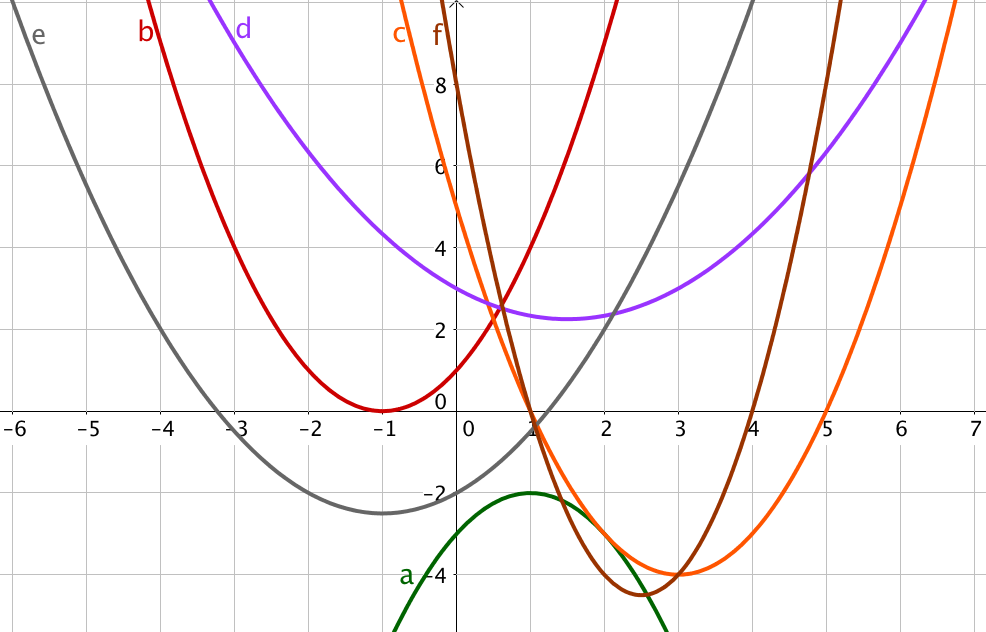
\includegraphics[width=0.4\textwidth]{img-sol/t5-14}}

\exer Un objecte es llança verticalment cap amunt des d'un determinat punt. L'altura en metres aconseguida al cap de $t$ segons, ve donada per $h(t)=5+4t-t^{2}$. Calcula l'altura des de la qual es llança l'objecte i a la qual es troba després d'1 segon. Determina en quin instant aconseguirà l'altura màxima i quina és. Finalment, calcula l'instant en què caurà al terra i representa gràficament la situació amb les dades obtingudes anteriorment.

\answers{L'objecte es llança des d'una altura de 5 m. Al cap d'1 s està a 8 m. Assoleix una altura màxima de 9 m als 2 s. Arriba al terra als 5 segons.\par 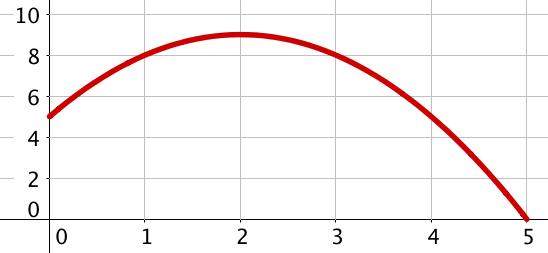
\includegraphics[width=0.4\textwidth]{img-sol/t5-15}}

\exer La despesa pel consum de llum (en cèntims d'euro) d'un habitatge, en funció del temps transcorregut (en hores), ens ve donada per l'expressió $f\left(t\right)\, \, =\, \, -\frac{1}{5} t^{2} +2t+10$ per a $0\le t\le 12$.

\begin{tasks}
\task Representa gràficament la funció.
\task Quin és el consum a les 6 hores? I després de 12 hores? 
\end{tasks}

\answers{a) \par 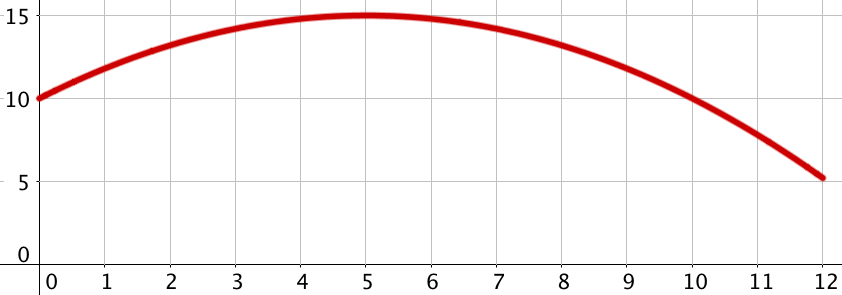
\includegraphics[width=0.4\textwidth]{img-sol/t5-16} \par b) $f(6)=14.8$ i $f(12)=5.2$ cèntims.}

\end{mylist}

\subsection{Funcions arrel}

\begin{mylist}
 \exer Representa gràficament les funcions:
 \begin{tasks}(4)
 	\task $y=\sqrt{x-1}$
 	\task $y=-\sqrt{x+3}$
 	\task $y=2+\sqrt{x}$
 	\task $y=1-\sqrt{x}$
\end{tasks}
\answers{\mbox{}\par 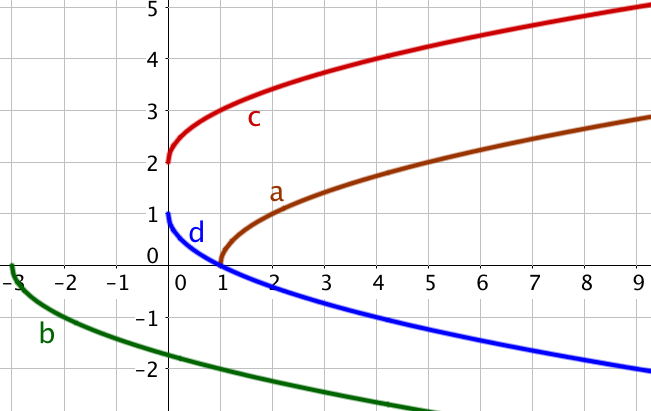
\includegraphics[width=0.4\textwidth]{img-sol/t5-17}}

\end{mylist}

\subsection{Proporcionalitat inversa (Hipèrboles)}
\begin{mylist}
 \exer Representa gràficament les funcions:
\begin{tasks}(4)
	\task $y=\dfrac{1}{x+1}$
	\task $y=\dfrac{1}{x-1}$
	\task $y=\dfrac{-1}{x}$
	\task $y=\dfrac{-1}{x-3}$
\end{tasks}
\answers{\mbox{}\par 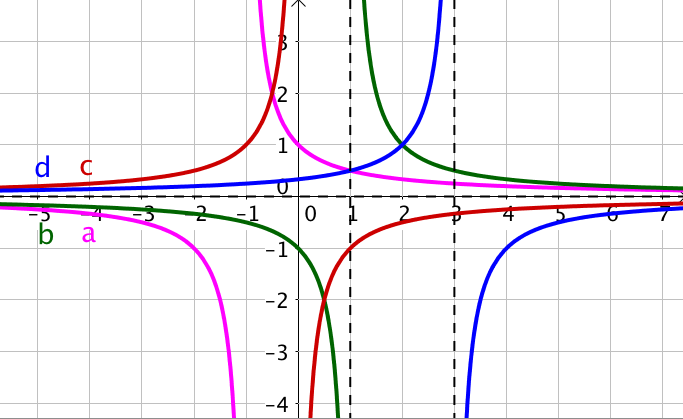
\includegraphics[width=0.4\textwidth]{img-sol/t5-18}}

\exer Dibuixa el recinte limitat pels semieixos positius de coordenades i les corbes $y=x^{2} +1,{\rm \; }y=\dfrac{2}{x} $ i  $y=x-1$.
\answers{\mbox{}\par 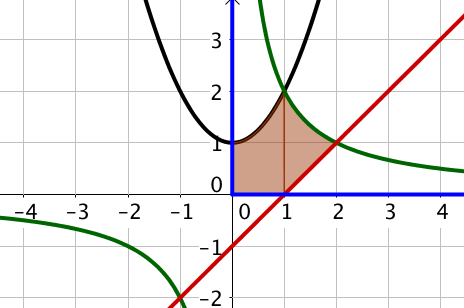
\includegraphics[width=0.4\textwidth]{img-sol/t5-19}}

\exer Els beneficis d'una empresa, en milers d'euros, s'ajusten a la funció $f\left(x\right)=\dfrac{50x-100}{2x+5} $, on $x$ representa els anys de vida de l'empresa, essent $x\ge 0$. Calcula el domini, tall amb els eixos, signe i simetries d'aquesta funció.

\answers{Dom $f=[0,+\infty]$. Tall eix OX $(2,0)$;  Tall eix OY $(0,-20)$. No presenta simetries. La funció és negativa a $[0,2)$ i positiva a $(2,+\infty)$.}
\end{mylist}

\subsection{Funció a trossos i valor absolut}
\begin{mylist}
	\exer  Representa gràficament la funció valor absolut $y=|x|$. Expressa-la com una funció a trossos.
	
	\answers{$|x|=\left\{ \begin{array}{ll}
		-x & \text{ si } x<0 \\
		 x & \text{ si } x\ge 0 
		\end{array} \right.$}
	
	\exer  Representa les següents funcions a trossos. 
	
	\begin{tasks}
	\task  $f(x)=\left\{\begin{array}{cl} x^{2} -1\; \; \; \;& si\; \; x<-4 \\ -x+2\; \; \; \;& si\; \; -4\le x<0 \\ 5\; \; \; \;& si\; \; \; \; 0\le x \end{array}\right. $  
	%
	\task  $g(x)=\left\{\begin{array}{cl} \frac{1}{x} \; \;& si\; \; x<-3 \\ x\; \; \; & si\; \; -3\le x<2 \\ \sqrt{x} \; \; \; \;& si\; \; 2\le x \end{array}\right. $  
	%
	\end{tasks}
\answers{\mbox{}\par 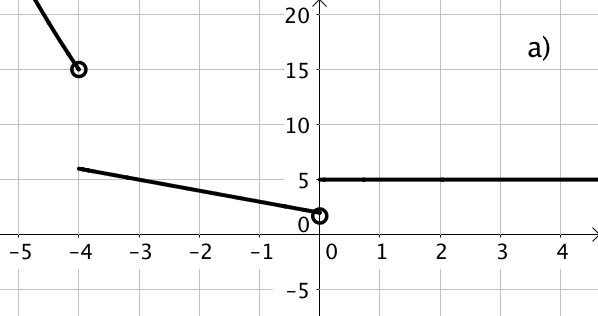
\includegraphics[width=0.4\textwidth]{img-sol/t5-22a}\par
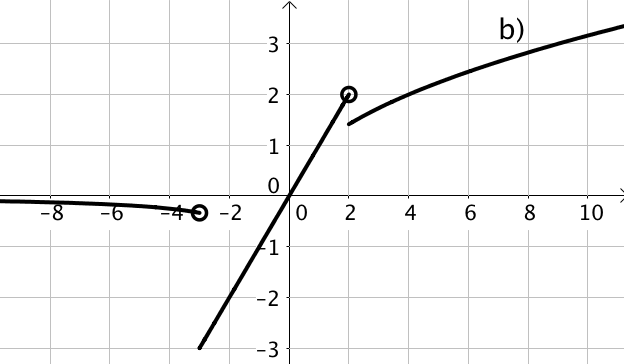
\includegraphics[width=0.4\textwidth]{img-sol/t5-22b}}


\exer Esbossa la gràfica de la funció $f$: $\Re$ $\rightarrow$ $\Re$ donada per $f(x)=\left\{\begin{array}{l} {2x+2\quad {\rm si\; \; }x\le -1,} \\ {x^{3} -x\quad {\rm si\; \; }x>-1.} \end{array}\right. $
\answers{\mbox{}\par 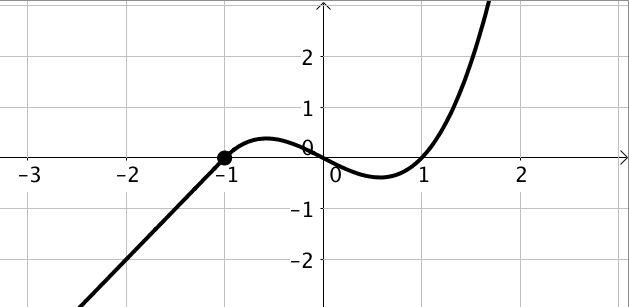
\includegraphics[width=0.4\textwidth]{img-sol/t5-23}}

\exer Siguin les funcions definides mitjançant $f(x){\rm \; }=\left|x\left(x-2\right)\right|$ i  $g(x)=x+4$. Representa les gràfiques de $f$ i $g$ sobre els mateixos eixos i calcula els punts de tall entre ambdues.
\answers{\mbox{}\par 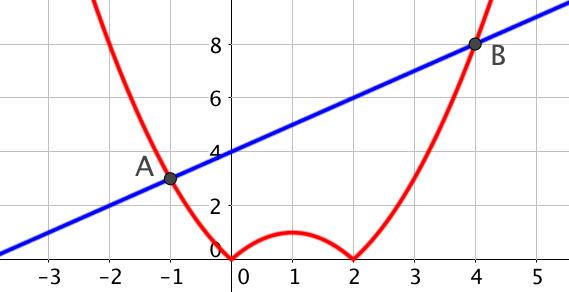
\includegraphics[width=0.4\textwidth]{img-sol/t5-24}}

\exer Representa les següents funcions i defineix-les com a funcions a trossos:
\begin{tasks}(4)
	\task $y=|4-x|$
	\task $y=|3x+6|$
	\task $y=|x^2-1|$
	\task $y=|x^2+2x-3|$
\end{tasks}
\answers{\mbox{}\par 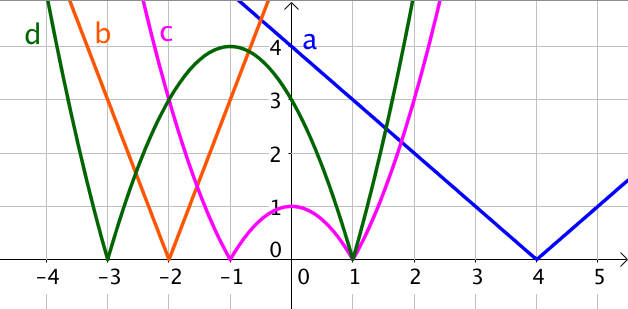
\includegraphics[width=0.4\textwidth]{img-sol/t5-25}}

\exer Sigui la funció $f(x)=\left\{\begin{array}{l} {1-x^{2} } \\ {3x^{2} -12x+9} \\ {-2x^{2} +16x-30} \end{array}{\rm \; \; \; \; }\begin{array}{c} {{\rm si}} \\ {{\rm si}} \\ {{\rm si}} \end{array}\right. {\rm \; \; \; }\begin{array}{l} {x\le 1} \\ {1<x\le 3} \\ {x>3} \end{array}$. Dibuixa la seva gràfica i, a partir d'ella, indica el seu domini, els  punts de tall amb els eixos i el seu signe.
\answers{\mbox{}\par 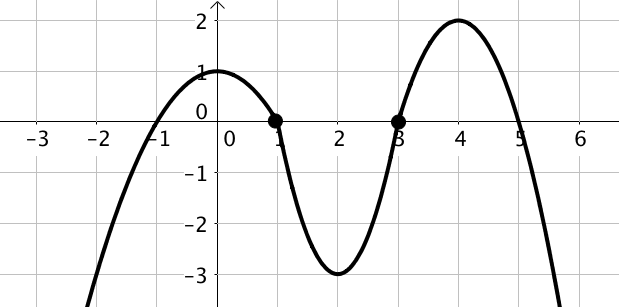
\includegraphics[width=0.4\textwidth]{img-sol/t5-26}}

\end{mylist}

\pagebreak
\subsection{Funció exponencial}

\begin{theorybox}
	Les funcions exponencials són del tipus $y=a^x$. Si $a>1$ són creixents i si $0<a<1$ són decreixents. Totes elles passen pel punt $(0, 1)$.
	
	Un cas important és $y=e^x$ on la base és el número $e \simeq 2.7182818$.
\end{theorybox}

\begin{mylist}
\exer  En el teu quadern, representa conjuntament les gràfiques de $y=f(x)=x^2$ (funció potencial) i $f(x)=2^x$ (funció exponencial), amb valors de ``\textit{x}'' entre 0 i 5. Observa la diferència quantitativa entre el creixement potencial i el creixement exponencial. 

\exer Dibuixa el recinte limitat per les corbes $y=e^{x+2} ,$ $y=e^{-x} $  i  $x=0.$
\answers{\mbox{}\par 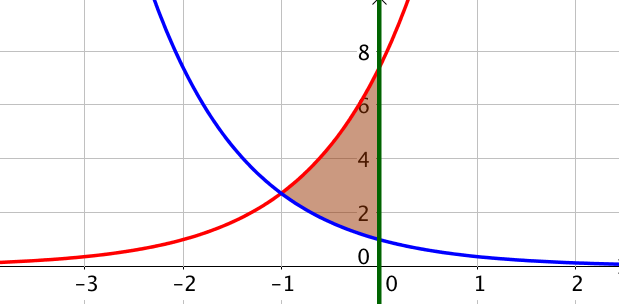
\includegraphics[width=0.4\textwidth]{img-sol/t5-28}}

\exer  Utilitzant la calculadora, fes en el teu quadern una taula de valors i representa les funcions \textit{f}(\textit{x}) = \textit{e${}^{x}$}  i \textit{g}(\textit{x}) = \textit{e${}^{-}$${}^{x}$}.
\answers{Són simètriques respecte l'eix OY.}

\exer  Una persona ha ingressat una quantitat de 5.000 euros a interès del 2 \% en un banc, de manera que cada any la seva capital es multiplica per 1'02.
\begin{tasks}
\task  Escriu en el teu quadern una taula de valors amb els diners que tindrà aquesta persona al cap d'1, 2, 3, 4, 5 i 10 anys.
%%
\task  Indica la fórmula de la funció que expressa el capital en funció del nombre d'anys.
%%
\task  Representa en el teu quadern gràficament aquesta funció. Pensa bé quines unitats hauràs d'utilitzar en els eixos.
\end{tasks}
\answers{[\mbox{}\par\begin{tabular}{|c|c|c|c|c|c|c|}
		anys & 1 & 2 & 3 & 4 & 5 & 10 \\ \hline
	 k\euro{} & 5.1 & 5.202 & 5.306 & 5.41 & 5.52 & 6.09
	\end{tabular},
	$C=5\cdot 1.02^x$
]}


%%
\exer  Un determinat antibiòtic fa que la quantitat de certs bacteris es multipliqui per 1/3 cada hora. Si la quantitat a les 9 del matí és de 10 milions de bacteris: 
 
 \begin{tasks}
\task Fes una taula calculant el nombre de bacteris que hi ha cada hora, des de les 3 del matí a les 12 de migdia (observa que has de calcular també ``cap a enrere'').
%
\task Representa gràficament aquestes dades.
\end{tasks}
\answers{$y=10\cdot \left(\frac{1}{3}\right)^x$, $x$ hores passades des de les 9 del matí. A les 3 del matí $y(-6)=7290$ i a les 12 del migdia $y(3)=0.37$ milions.}

\end{mylist}

\section{Composició de funcions. Funció inversa.}

\begin{example}
Donades les funcions $f(x)=e^x$ i $g(x)=\dfrac{1}{\cos x}$, demanen calcular les composicions $(f\circ g)(x)$ i $(g\circ f)(x)$:
	
	La composició $f\circ g = f[g(x)]=f\left[\frac{1}{\cos x}\right]=e^{\frac{1}{\cos x}}$.
	
	En canvi, la composició  $g\circ f = g[f(x)]=g\left[e^x\right]=\dfrac{1}{\cos (e^x)}$.
\end{example}

\vspace{5cm}
\begin{theorybox}[Procediment per calcular $f^{-1}(x)$]	
	Les funcions $f$ i $f^{-1}$ són inversa una de l'altre si es compleixen les composicions 
	%%
	\[ f[f^{-1}(x)]=f^{-1}[f(x)]=x \]
 
	Si ens donen la funció $y=\dfrac{2x}{x+1}$ i volem calcular la seva funció inversa, començam canviant el nom de les variables $x \leftrightarrows y$.
	
	Ara hem d'aïllar $y$ de l'expressió $x=\dfrac{2y}{y+1}$. Trobam $y=\dfrac{x}{2-x}$ i aquesta és la funció inversa $f^{-1}(x)$.
\end{theorybox}

\begin{mylist}
\exer Considerem les següents funcions:
 
\begin{tabular}{|p{1.64in}|p{1.65in}|p{1.65in}|} \hline 
 $f(x)=x^{3} -3x^{2} +3x-1$ & $g(x)=\sqrt[{}]{\frac{x-2}{x+7} }$ & $h(x)=2^{-x+1}$ \\ \hline
  $j(x)=\ln \left(x^{5} -1\right)$ & $k(x)=2^{x} \, \cdot \, 30^{x-1}$ & $m(x)=\sqrt[{4}]{-5+2x}$ \\
  \hline 
\end{tabular}


\begin{tasks}
\task Calcula les següents composicions:
$f\circ h$; $g\circ h$; $g\circ j$; $k\circ h$; $g\circ h \circ j$; $m\circ j$
\task Calcula $f^{-1} \left(x\right),{\rm \; }h^{-1} \left(x\right),{\rm \; }k^{-1} \left(x\right),{\rm \; }j^{-1} \left(x\right)$ i verificar que són les inverses de $f\left(x\right),{\rm \; }h\left(x\right),{\rm \; }k\left(x\right),{\rm \; }j\left(x\right){\rm \; }$.  
%
\task Calcula tots els dominis.
%
\task Calcula els punts de tall amb els eixos de totes les funcions.
\end{tasks}

\answers{[$f\circ h=2^{-3x+3}-3\,2^{-2x+2}+3\,2^{-x+1}-1$;\par $g\circ h=\sqrt{\frac{2^{-x+1}-2}{2^{-x+1}+7}}$;\par $g\circ j=\sqrt{\frac{\ln(x^5-1)-2}{\ln(x^5-1)+7}}$;\par $k\circ h=2^{2^{-x+1}}\cdot 30^{2^{-x+1}-1}$;\par   $g\circ h \circ j=\sqrt{\frac{2^{-\ln(x^5-1)+1}-2}{2^{-\ln(x^5-1)+1}+7}}$;\par $m\circ j=\sqrt[4]{-5+2\ln(x^5-1)}$,
Dom $f=\Re$; Dom $g=(-\infty,-7)\cup[2,+\infty]$; Dom $h=\Re$; Dom $j=(1,+\infty)$; Dom $k=\Re$; Dom $m=[5/2,+\infty]$]}


\exer[1] Calcula en el teu quadern les inverses (que existeixin) de les funcions següents:
\[\begin{array}{llll} 
p(x)=-5x+3\quad &\quad q(x)=2x^{2} - 1\quad & \quad r(x)=-x^{3} +6\quad & \quad s(x)=-x \\ 

f(x)=\frac{2x-4}{x+3} \quad & \quad g(x)=\frac{-3}{x} \quad & \quad h(x)=\frac{x+1}{x^{2} } \quad &\quad j(x)=\frac{-x^{2} }{x^{2} -4} \\ 

k(x)=e^{x-4} \quad &\quad l(x)=2^{\frac{1}{x} } \quad & \quad m(x)=\left(\frac{2}{3} \right)^{x} \quad & \quad n(x)=e^{\frac{x}{x-1} }  \\

 a(x)=\ln \left(x-2\right)\quad & \quad b(x)=\log \left(\frac{x-1}{3} \right)\quad & \quad c(x)=\ln \left(\frac{x -1}{2x+4} \right)\quad & \quad d(x)=\log \left(x^{3} -1\right)
 
  \end{array}\] 
  
 \begin{comment}
\begin{tabular}{|p{0.2in} p{0.7in}|p{0.9in}|p{0.6in}|p{0.2in} p{0.7in}|p{1.5in}|} \hline 
\multicolumn{2}{|p{1in}|}{\textbf{FUNCIÓ}} & \multicolumn{2}{|p{1.5in}|}{\textbf{INVERSA}} & \multicolumn{2}{|p{0.9in}|}{\textbf{FUNCIÓ}} & \textbf{INVERSA} \\ \hline 
\textit{} & $p(x)$ & \multicolumn{2}{|p{1.5in}|}{} &  \textit{} & $q(x)$ &  \\ \hline 
\textit{} & $r(x)$ & \multicolumn{2}{|p{1.5in}|}{} &  \textit{} & $s(x)$ &  \\ \hline 
\textit{} & $f(x)$ & \multicolumn{2}{|p{1.5in}|}{} &  \textit{} & $g(x)$ &  \\ \hline 
\textit{} & $h(x)$ & \multicolumn{2}{|p{1.5in}|}{} &  \textit{} & $j(x)$ &  \\ \hline 
\textit{} & $k(x)$ & \multicolumn{2}{|p{1.5in}|}{} &  \textit{} & $l(x)$ &  \\ \hline 
\textit{} & $m(x)$ & \multicolumn{2}{|p{1.5in}|}{} &  \textit{} & $n(x)$ &  \\ \hline 
\textit{} & $a(x)$ & \multicolumn{2}{|p{1.5in}|}{} &  \textit{} & $b(x)$ &  \\ \hline 
\textit{} & $c(x)$ & \multicolumn{2}{|p{1.5in}|}{} &  \textit{} & $d(x)$ &  \\ \hline 
\end{tabular}
\end{comment}
\answers{$p^{-1}=(3-x)/5$,\par $q^{-1}=\pm \sqrt{(x+1)/2}$,\par $r^{-1}=\sqrt[3]{6-x}$, $s^{-1}=-x$,\par $f^{-1}=(3x+4)/(2-x)$, $g^{-1}=-3/x$,\par $h^{-1}=(1\pm \sqrt{1+4x})/2$,\par $j^{-1}=\pm \sqrt{4x/(1+x)}$, \,\,$k^{-1}=4+\ln x$,\par $l^{-1}=1/\log_2 {x}$,\par $m^{-1}=\log x /(\log 2 - \log 3)$,\par $n^{-1}=\ln x  / (\ln x -1)$,\par $a^{-1}=2+e^x$, $b^{-1}=3\cdot 10^x +1$,\par $c^{-1}=(1+4 e^x)/(1-2 e^x)$,\par $d^{-1}=\sqrt[3]{1+10^x}$ }


\exer  Calcula la funció inversa de la funció lineal representada:

\begin{center}
	  \includegraphics*[width=2.1in]{img-05/ex24-fe.pdf}
\end{center}

\answers{La funció representada és la recta $y=-\frac{3}{5}x+3$. La seva inversa és $y=-\frac{5}{3}x+5$}

\end{mylist}

\pagebreak
\section{Logaritmes}

\subsection{Definició de logaritme}
\begin{theorybox}
	
	\begin{minipage}{0.7\textwidth}
		\begin{equation*}
			\log_b y = x  \quad \leftrightarrow \quad b^x = y
		\end{equation*}
	\end{minipage}
	\begin{minipage}{0.3\textwidth}
		
\includegraphics[width=0.5\textwidth]{img-05/log-calculadora}
	\end{minipage}
	
	$b$ és la base del logaritme, que ha d'ésser positiva i diferent de 1. Si la base és 10, tenim el logaritme decimal $\log_{10} x= \log x$. Si en canvi triam com a base el número $e=2.7182818\cdots$, obtenim el logaritme Neperià, $\log_e x= \ln x$
\end{theorybox}

\begin{mylist}
	\exer Calcula la base d'aquests logaritmes:
	\begin{tasks}(3)
		\task $\log_x 125 = 3$
		\task $\log_x \frac{1}{9}=-2$
		\task $\log_x \frac{1}{4} = 2$
		\task $\log_x 2 =\frac{1}{2}$
		\task $\log_x 0,04 = -2$
		\task $\log_x 4 = -\frac{1}{2}$
		\end{tasks}

\answers{[$x=5$, $x=3$, $x=\frac{1}{2}$, $x=4$, $x=5$, $x=\frac{1}{16}$]}

	\exer Calcula el valor de $x$:
\begin{tasks}(3)
	\task $\log x^2 = -2$
	\task $7^x = 115$
	\task $\log_7 3x = 0,5$
	\task $3^{2+x} = 172$
	\task $\ln x = 2$
	\task $\log_2 \sqrt{8}=x$
\end{tasks}

\answers{[$x=\pm\frac{1}{10}$, $x=\log_7 115\approx 2,438$, $x=\frac{\sqrt{7}}{3}\approx 0,882$, $x=-2+\log_3 172\approx 2,685$, $x=e^2\approx 7,389$, $x=\frac{3}{2}$]}

\end{mylist}

\subsection{Propietats dels logaritmes}


\begin{mylist}
	\exer[1]  Utilitza les propietats dels logaritmes per resoldre aquestes equacions:
	\begin{tasks}(2)
		\task $\log x^2 + \log 2 - \log x - \log 3 = 1$
		\task $(2^{x+1})^2 = 64$
		\task $2\log x = 3 +\log \frac{x}{10}$
		\task $2^x = 10^{x+2}$
		\task $\dfrac{\ln(16-x^2)}{\ln(3x-4)}=2$
		\task $9^{x+1} + 3 = 28\cdot 3^x$
	\end{tasks}
\answers[cols=1]{[$x=15$ ($x=0$ no vàlida), $x=2$, $x=100$ ($x=0$ no vàlida), $x=2/(\log 2 - 1)$, $x=12/5$,  $x=1$ i $x=-2$]}

\end{mylist}

\begin{theorybox}[Propietats dels logaritmes]
 \begin{enumerate}
 	\item \label{eq:proplog} $\log_b 1 = 0$
 	\item $\log_b b = 1$
	\item $\log_b (A \cdot B) =  \log_b A + \log_b B$
	\item $\log_b A^n = n \log_b A$
	\item $\log_b \left( \frac{A}{B} \right) = \log_b A - \log_b B$
	\item $\log_b A = \dfrac{\log A}{\log b}$      \quad   \textit{Fórmula del canvi de base}	
 \end{enumerate}
\end{theorybox}




\subsection{La funció logarítmica}

\begin{mylist}
\exer  Identifica les fórmules de les següents funcions a partir de les seves gràfiques, sabent que són funcions logarítmiques:

\includegraphics*[width=1.4in]{img-05/ex25fe-a}
\includegraphics*[width=1.4in]{img-05/ex25fe-b} 
\includegraphics*[width=1.4in]{img-05/ex25fe-c}
\includegraphics*[width=1.4in]{img-05/ex25fe-d}


\answers{[$y=\log_4 x$, $y=\ln x$, $y=\log_{1/4} x=-\log_4 x$, $y=\log_{1/e} x=-\ln x$]}

\exer  Representa en el teu quadern, mitjançant taules de valors, les gràfiques de les següents funcions:
\begin{tasks}(3)
\task  $f(x)=\log _{3} x$ \task  $f(x)=\log _{1/3} x$  \task  $f(x)=\log _{1,5} x$
\end{tasks}

Comprova que en tots els casos passen pels punts (1, 0), (\textit{b}, 1) i (1/\textit{b}, $-1$), on \textit{b} és la base.

\answers{\mbox{}\par 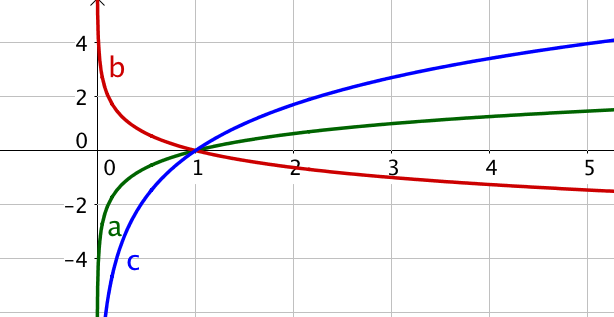
\includegraphics[width=0.4\textwidth]{img-sol/t5-39}}

\exer Considera la funció definida per $\; f\left(x\right)=\dfrac{2\log x}{x^{2} } $ . Calcula el seu domini.
\answers{Dom $f=(0,+\infty)$}

\exer Considera la funció definida per $g\left(x\right)=\left|\ln\left(x\right)\right|$ (on ln denota el logaritme neperià). Esbossa el recinte limitat per la gràfica de $g$ i la recta $y = 1$. Calcula els punts de tall entre elles.

\answers{Punt de tall $A(e,1)$ i $B(1/e,1)$ \par 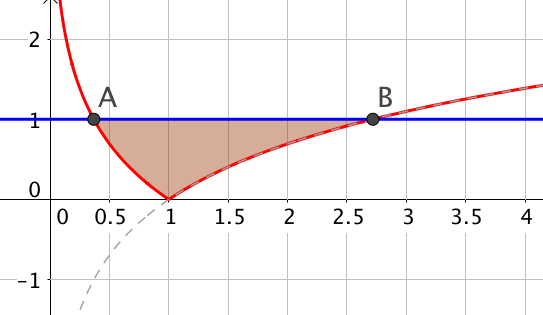
\includegraphics[width=0.4\textwidth]{img-sol/t5-41}}

\exer Calcula el domini de les següents funcions: $f(x)=\dfrac{{\rm \ln}x}{x^{2} }$, $g(x)=(1-x^{3} )\cos x$ i $h(x)=4x^{3} -5x+\frac{1}{e^{x} } $.

\answers{Dom $f=(0,+\infty)$; Dom $g=\Re$; Dom $h=\Re$}

\end{mylist}
 

\section{Funcions trigonomètriques}

\begin{theorybox}
	Les funcions $y=\sin x$, $y=\cos x$ i $y=\tg x$ són funcions periòdiques o circulars de període $2\pi$, $2\pi$ i $\pi$ respectivament.
	
	
\includegraphics[width=0.8cm]{img-05/warning} \textbf{ Recorda que la $x$ ve donat en radiants en les funcions trigonomètriques.} 
\end{theorybox}

\begin{mylist}
	\exer Representa la funció $f(x)=\sin x$  entre $x=-\pi$ i $x=2\pi$.
	\answers{\mbox{}\par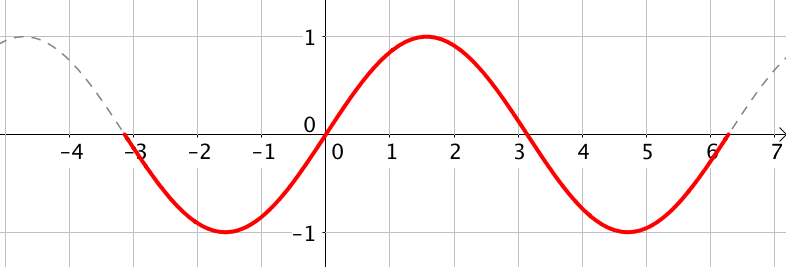
\includegraphics[width=0.4\textwidth]{img-sol/t5-43}}
	
	\exer Considera les funcions $f$, $g$: [0, $2\pi$] $\rightarrow$ $\Re$, $f(x)=2\cdot  \sin(x)$  i  $g(x)=\sin(2x).$ Dibuixa la regió del pla limitada per les gràfiques de $f$ i $g$.
	\answers{\mbox{}\par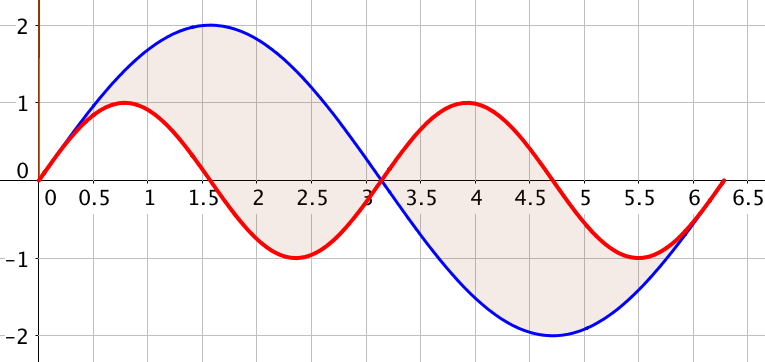
\includegraphics[width=0.4\textwidth]{img-sol/t5-44}}

\exer Representa la funció $f(x)=\cos x + \frac{1}{2} \cos 2x$ entre $x=0$ i $x=\pi/4$.
\answers{\mbox{}\par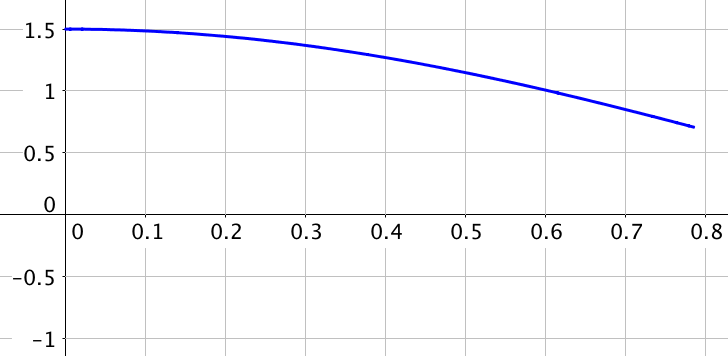
\includegraphics[width=0.4\textwidth]{img-sol/t5-45}}

\exer La posició d'una bolla que es troba enganxada a l'extrem d'una molla, oscil·la d'acord amb l'equació $x=10\sin\left(\frac{2\pi }{5}t + \frac{\pi}{2}\right)$. Construeix una taula de valors i representa la funció $x(t)$.
\answers{\mbox{}\par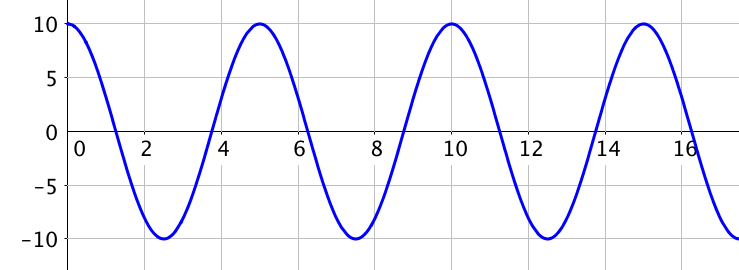
\includegraphics[width=0.4\textwidth]{img-sol/t5-46}}
\end{mylist}

\newpage
\begin{autoaval}{55}

\begin{mylist}
\exer[2] L'expressió de la composició $f\circ g$ de les funcions $f(x)=2x-1$ i $g(x)=-x^2+2$ és:
	\begin{tasks}(4)
		\task $-2x^2+3$
		\task $2x^2-3$
		\task $-4x^2+4x+1$
		\task $4x^2-4x-1$
		\end{tasks}
	\answers{\textbf{-- 10.} Autoavaluació: 1a; 2d; 3d; 4b; 5c; 6b; 7b; 8a; 9c; 10c}

\exer La funció inversa de $f(x)=\frac{x-1}{x+1}$ és:
\begin{tasks}(4)
	\task $\frac{x+2}{x-1}$
	\task $\frac{-x+1}{x+2}$
	\task $\frac{2x+1}{x-1}$
	\task $\frac{-2x-1}{x-1}$
\end{tasks}

\exer La funció inversa de $f(x)=2+\ln x$ és:
\begin{tasks}(4)
	\task $\frac{1}{2 + \ln x}$
	\task $2+\ln (-x)$
	\task $e^{x}+2$
	\task $e^{x-2}$
\end{tasks}

\exer La paràbola $y=-x^2+2x+3$ és:
	\begin{tasks}(2)
	\task Convexa i té un màxim a $(0,3)$
	\task Convexa i té un màxim a $(1,4)$
	\task Còncava i té un mínim a $(1,4)$
	\task Còncava i té un mínim a $(0,3)$
\end{tasks}

\exer El domini de la funció $f(x)=e^{\frac{x}{x^2-1}}$ és:
	\begin{tasks}(4)
	\task $\mathbb{R}$
	\task $\mathbb{R}-\{1\}$
	\task $\mathbb{R}-\{-1,1\}$
	\task $\mathbb{R}-\{0\}$
	\end{tasks}


\exer El domini de la funció $f(x)=\sqrt{1-x^2}$ és:
\begin{tasks}(4)
	\task $(-1,1)$
	\task $[-1,1]$
	\task $\mathbb{R}-\{-1,1\}$
	\task $(-\infty,-1]\cup[1,+\infty)$
\end{tasks}

\exer Els punts de tall de la funció $f(x)=\ln(x^2-3x+3)$ amb l'eix de les abscisses són:
	\begin{tasks}(4)
	\task No en té
	\task (1, 0); (2, 0)
	\task (-1, 0); (2, 0)
	\task (0, $\ln 3$)
\end{tasks}

\exer La gràfica de la funció $y=\log_{2} x$ és:
\begin{tasks}(4)
	\task  \includegraphics*[width=2cm]{img-05/chap-fe-autoaval-opta}
	\task  \includegraphics*[width=2cm]{img-05/chap-fe-autoaval-optb}
	\task  \includegraphics*[width=2cm]{img-05/chap-fe-autoaval-optc}
	\task  \includegraphics*[width=2cm]{img-05/chap-fe-autoaval-optd}
\end{tasks}


\exer La gràfica de la funció $y=\left\{\begin{array}{ll} 
		\sqrt{1-x} & x<-1 \\ \frac{1}{x} & -1 \leq x <0 \\ 2^x & x\geq 0
	 \end{array}  \right.$ és:
\begin{tasks}(4)
	\task  \includegraphics*[width=2cm]{img-05/chap-fe-autoaval-eea}
	\task  \includegraphics*[width=2cm]{img-05/chap-fe-autoaval-eeb}
	\task  \includegraphics*[width=2cm]{img-05/chap-fe-autoaval-eec}
	\task  \includegraphics*[width=2cm]{img-05/chap-fe-autoaval-eed}
\end{tasks}

\exer L'única funció NO periòdica de les següents és:
\begin{tasks}(4)
	\task $y=\sin x$
	\task $y=\tg x$ 
	\task  $y=\cos(e^x) $
	\task  $y=e^{\cos x}$
\end{tasks}

\end{mylist}
\end{autoaval}

\newpage
\resum 
\begin{center}
\includegraphics[width=0.7\textwidth,angle=90,origin=c,page=3]{img-05/funcions-elementals}
\hspace{1cm}
\includegraphics[width=0.7\textwidth,angle=90,origin=c,page=4]{img-05/funcions-elementals}

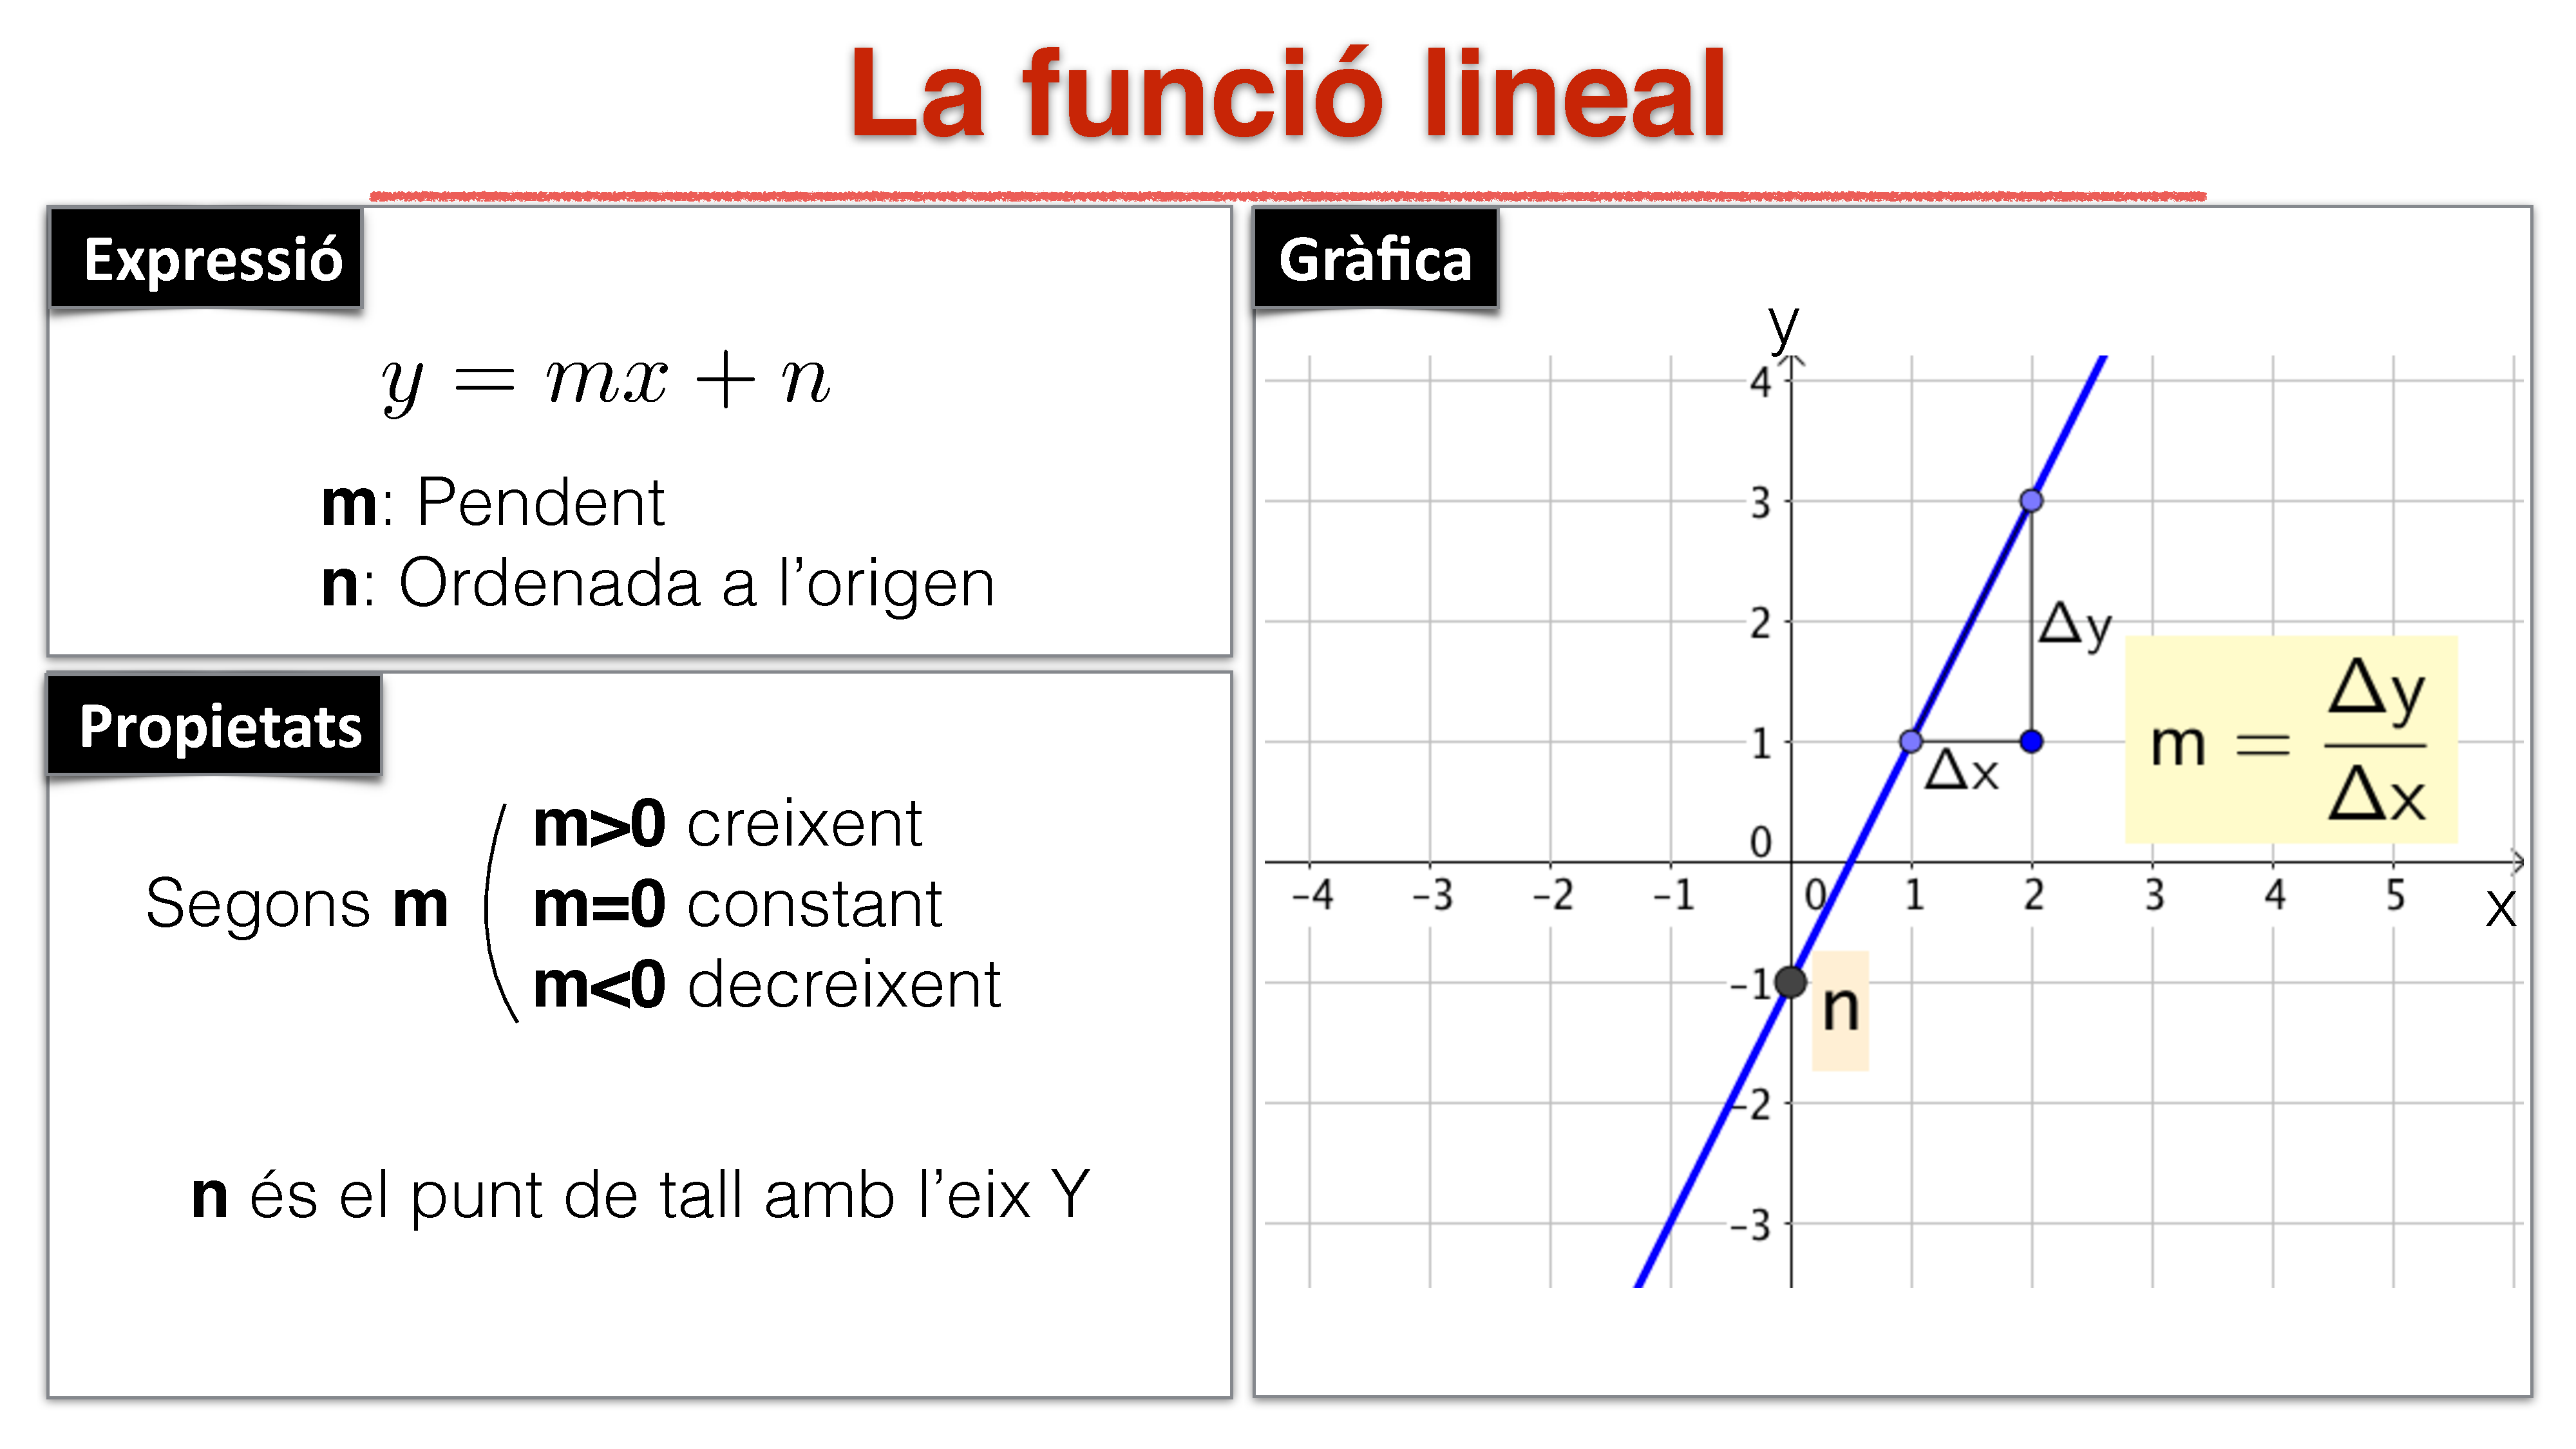
\includegraphics[width=0.7\textwidth,angle=90,origin=c,page=1]{img-05/funcions-elementals}
\hspace{1cm}
\includegraphics[width=0.7\textwidth,angle=90,origin=c,page=2]{img-05/funcions-elementals}
\end{center}

\begin{center}
\includegraphics[width=0.7\textwidth,angle=90,origin=c,page=7]{img-05/funcions-elementals}
\hspace{1cm}
\includegraphics[width=0.7\textwidth,angle=90,origin=c,page=8]{img-05/funcions-elementals}

\includegraphics[width=0.7\textwidth,angle=90,origin=c,page=5]{img-05/funcions-elementals}
\hspace{1cm}
\includegraphics[width=0.7\textwidth,angle=90,origin=c,page=6]{img-05/funcions-elementals}
\end{center}
 
